% !TEX TS-program = XeLaTeX
% use the following command:
% all document files must be coded in UTF-8
\documentclass[english]{textolivre}
% build HTML with: make4ht -e build.lua -c textolivre.cfg -x -u article "fn-in,svg,pic-align"

\journalname{Texto Livre}
\thevolume{16}
%\thenumber{1} % old template
\theyear{2023}
\receiveddate{\DTMdisplaydate{2023}{3}{1}{-1}} % YYYY MM DD
\accepteddate{\DTMdisplaydate{2023}{4}{20}{-1}}
\publisheddate{\DTMdisplaydate{2023}{8}{2}{-1}}
\corrauthor{Jefferson Rodrigues-Silva}
\articledoi{10.1590/1983-3652.2023.44946}
%\articleid{NNNN} % if the article ID is not the last 5 numbers of its DOI, provide it using \articleid{} commmand 
% list of available sesscions in the journal: articles, dossier, reports, essays, reviews, interviews, editorial
\articlesessionname{articles}
\runningauthor{Rodrigues-Silva and Alsina} 
%\editorname{Leonardo Araújo} % old template
\sectioneditorname{Daniervelin Pereira}
\layouteditorname{Thaís Coutinho}

\title{Conceptualising and framing STEAM education: what is (and what is not) this educational approach?}
\othertitle{Conceitualização e modelo da educação STEAM: o que é (e o que não é) essa abordagem educacional?}
% if there is a third language title, add here:
%\othertitle{Artikelvorlage zur Einreichung beim Texto Livre Journal}

\author[1]{Jefferson Rodrigues-Silva~\orcid{0000-0002-8334-2107}\thanks{Email: \href{mailto:jeffe.rodri@gmail.edu.br}{jeffe.rodri@gmail.edu.br}}}
\author[2]{Ángel Alsina~\orcid{0000-0001-8506-1838}\thanks{Email: \href{mailto:angel.alsina@udg.edu}{angel.alsina@udg.edu}}}
\affil[1]{Federal Institute of Minas Gerais, Department of Mechanical Engineering, Arcos, Minas Gerais, Brazil.}
\affil[2]{University of Girona, Department of Subject-Specific Didactics, Girona, Catalonia, Spain.}

\addbibresource{article.bib}
% use biber instead of bibtex
% $ biber article

% used to create dummy text for the template file
\definecolor{dark-gray}{gray}{0.35} % color used to display dummy texts
\usepackage{lipsum}
\SetLipsumParListSurrounders{\colorlet{oldcolor}{.}\color{dark-gray}}{\color{oldcolor}}

% used here only to provide the XeLaTeX and BibTeX logos
\usepackage{hologo}

% if you use multirows in a table, include the multirow package
\usepackage{multirow}

% provides sidewaysfigure environment
\usepackage{rotating}

% CUSTOM EPIGRAPH - BEGIN 
%%% https://tex.stackexchange.com/questions/193178/specific-epigraph-style
\usepackage{epigraph}
\renewcommand\textflush{flushright}
\makeatletter
\newlength\epitextskip
\pretocmd{\@epitext}{\em}{}{}
\apptocmd{\@epitext}{\em}{}{}
\patchcmd{\epigraph}{\@epitext{#1}\\}{\@epitext{#1}\\[\epitextskip]}{}{}
\makeatother
\setlength\epigraphrule{0pt}
\setlength\epitextskip{0.5ex}
\setlength\epigraphwidth{.7\textwidth}
% CUSTOM EPIGRAPH - END

% LANGUAGE - BEGIN
% ARABIC
% for languages that use special fonts, you must provide the typeface that will be used
% \setotherlanguage{arabic}
% \newfontfamily\arabicfont[Script=Arabic]{Amiri}
% \newfontfamily\arabicfontsf[Script=Arabic]{Amiri}
% \newfontfamily\arabicfonttt[Script=Arabic]{Amiri}
%
% in the article, to add arabic text use: \textlang{arabic}{ ... }
%
% RUSSIAN
% for russian text we also need to define fonts with support for Cyrillic script
% \usepackage{fontspec}
% \setotherlanguage{russian}
% \newfontfamily\cyrillicfont{Times New Roman}
% \newfontfamily\cyrillicfontsf{Times New Roman}[Script=Cyrillic]
% \newfontfamily\cyrillicfonttt{Times New Roman}[Script=Cyrillic]
%
% in the text use \begin{russian} ... \end{russian}
% LANGUAGE - END

% EMOJIS - BEGIN
% to use emoticons in your manuscript
% https://stackoverflow.com/questions/190145/how-to-insert-emoticons-in-latex/57076064
% using font Symbola, which has full support
% the font may be downloaded at:
% https://dn-works.com/ufas/
% add to preamble:
% \newfontfamily\Symbola{Symbola}
% in the text use:
% {\Symbola }
% EMOJIS - END

% LABEL REFERENCE TO DESCRIPTIVE LIST - BEGIN
% reference itens in a descriptive list using their labels instead of numbers
% insert the code below in the preambule:
%\makeatletter
%\let\orgdescriptionlabel\descriptionlabel
%\renewcommand*{\descriptionlabel}[1]{%
%  \let\orglabel\label
%  \let\label\@gobble
%  \phantomsection
%  \edef\@currentlabel{#1\unskip}%
%  \let\label\orglabel
%  \orgdescriptionlabel{#1}%
%}
%\makeatother
%
% in your document, use as illustraded here:
%\begin{description}
%  \item[first\label{itm1}] this is only an example;
%  % ...  add more items
%\end{description}
% LABEL REFERENCE TO DESCRIPTIVE LIST - END


% add line numbers for submission
%\usepackage{lineno}
%\linenumbers

\begin{document}
\maketitle

\begin{polyabstract}
\begin{abstract}
STEAM is a recent educational approach intending the interdisciplinary teaching of science, technology, engineering, arts/humanities, and mathematics. The literature reports conceptual confusion that frequently diverts STEAM practice and research to issues concerning particular activities or contexts. Therefore, we carried out a narrative review of articles indexed in the Web of Science (WoS) to elucidate STEAM education’s history, epistemology, and divergences. As a strategy, we first focused on documents that could offer a panoramic view of the object of study – literature reviews and articles about STEAM frameworks. Through them, we identified essential discussion points and further expanded the review. As a result, we articulated rationalities about why STEAM is not a mere evolution of STEM, a teaching methodology, or just a synonym for interdisciplinarity. Furthermore, we discussed the appropriateness of interdisciplinarity in STEAM – since it is strongly supported by the disciplines and their intersections – instead of pursuing transdisciplinarity, meaning knowledge remains undefined in a holistic whole. We differentiated STEAM disciplines (list of the five knowledge areas), STEAM activities (interdisciplinary teaching unity of at least two STEAM disciplines), and STEAM education (educational approach of interdisciplinarity between all five disciplines). Finally, we defined and proposed a framework for STEAM in a table format that stresses two necessary and sufficient conditions – interdisciplinarity and the five acronym areas. The framework permits envisioning the plurality of teaching methodologies and educational objectives consistent with STEAM.

\keywords{Educational models \sep Integrated curriculum \sep Interdisciplinary approach}
\end{abstract}

\begin{portuguese}
\begin{abstract}
STEAM é uma abordagem educacional recente que visa o ensino interdisciplinar de ciência, tecnologia, engenharia, artes/humanidades e matemática. A literatura relata confusão conceitual que frequentemente desvia a prática e a pesquisa de STEAM para questões relacionadas a atividades ou contextos específicos. Portanto, realizamos uma revisão narrativa de artigos indexados em Web of Science (WoS) para elucidar a história, epistemologia e divergências da educação STEAM. Como estratégia, primeiro nos centramos em documentos que pudessem oferecer uma visão panorâmica do objeto de estudo – revisões da literatura e artigos que discutem modelos teóricos de STEAM. Identificamos junções essenciais de discussão e expandimos a revisão. Articulamos racionalidades sobre por que STEAM não é uma evolução do STEM, uma metodologia de ensino ou um sinônimo de interdisciplinaridade. Além disso, discutimos a adequação da interdisciplinaridade em STEAM, que é fortemente apoiada pelas disciplinas e suas interseções; em vez da transdisciplinaridade, em que o conhecimento permanece difuso dentro de um todo holístico. Diferenciamos os conceitos disciplinas STEAM (lista das cinco áreas de conhecimento), atividades STEAM (unidade de ensino interdisciplinar de pelo menos duas disciplinas STEAM) e a educação STEAM (abordagem educacional de interdisciplinaridade entre todas as cinco disciplinas). Finalmente, definimos e propusemos um modelo para STEAM em formato de mesa que destaca duas condições necessárias e suficientes – interdisciplinaridade e as cinco áreas do acrônimo. O modelo permite visualizar a pluralidade de metodologias de ensino e objetivos educacionais consistentes com STEAM.

\keywords{Modelos educacionais \sep Currículo integrado \sep Abordagem interdisciplinar}
\end{abstract}
\end{portuguese}
% if there is another abstract, insert it here using the same scheme
\end{polyabstract}

\section{Introduction}
Interdisciplinarity pedagogies have been advocated through the rationality that siloed knowledge cannot address complex and global issues \cite{perignat_steam_2019}. Following this, the United States of America (USA) forged the acronym STEM in the 90s, referring to the integration of science, technology, engineering, and mathematics. Alternatively, STEAM emerged, considering science, technology, engineering, arts/humanities, and mathematics \cite{chesky_introduction_2015}.

Since their formalisation, STEM and STEAM have progressed in research and practice as interdisciplinary approaches between the areas circumscribed in each acronym. They incorporate current critical knowledge, such as technology and engineering, traditionally absent from pre-college levels. Bibliometric studies confirm they have advanced as research lines in education \cite{marin-marin_steam_2021}. Several countries, e.g., the USA, Korea, and Spain, have embraced them in their curriculums \cite{korea2013, ministerio2022real, ngss1900next}. The literature reports experiences in STEM or STEAM that mention successful outcomes in integrating knowledge areas and developing sustainable concerns such as environmental protection, food literacy, and gender equity \cite{costa-lizama_hack4women:_2022, silva-hormazabal_conectando_2022, stephenson_increasing_2022}.

Despite the enthusiasm, STEM and STEAM face criticism and epistemological divergences. The bifurcation of the acronyms itself signals those divergencies. STEM and STEAM represent contrary lines of narrowing the curriculum into technical areas or broadening it with arts and humanities. In the first direction, researchers defend that the expansion of STEM weakens the coherence of technical areas \cite{clements_stem_2021}. Contrarily, other researchers intend to broaden the curriculum through the non-exclusion of arts and humanities. The latter propose STEAM precisely to prevent the concentration or privilege of technical areas \cite{perignat_steam_2019}.

Specifically addressing STEAM, this educational approach is embedded in contemporary educational research and practice tendencies. For instance, STEAM is predominantly oriented toward the socio-constructivist paradigm and claims configurations such as active, collaborative, authentic, and meaningful learning \cite{schlesinger_cognitive_2020}. Practitioners frequently adopt active teaching methodologies such as Project-Based Learning (PjBL), Problem-Based Learning (PBL), and games \cite{aguilera_stem_2021}.

Literature reviews have focused on specific characteristics and contexts of STEAM, such as intertwined with playful learning or in Early Childhood Education for Sustainability (ECEfS) \cite{rodrigues-silva_predisposicoes_2022b, rodrigues-silva_educacion_2023a}. Meanwhile, there is a conceptual misunderstanding of what is essential in STEAM. In this vein, some studies propose frameworks for STEAM, but they incorporate features that restrict it to particularities of some educational settings, teaching methodologies, and contexts. There is a literature gap in a broader reflection on the distinctiveness of STEAM: what differentiates STEAM from a mere synonym of interdisciplinarity; what differentiates mentioning STEAM disciplines from single STEAM activities or the whole STEAM education.

Considering all that, we inquire – what is (and what is not) STEAM education. At the same time, we address the literature gap for comprehensive reviews and non-restrictive frameworks of STEAM. Accordingly, we aim to elucidate STEAM education’s history, epistemology, and divergences. Following, we pursue defining it and present a framework focusing on STEAM’s essential aspects.


\section{Methodology}

Reviews can be systematic or unsystematic – also called narrative reviews. Each type of review presents advantages and limitations. Complementarly, they help make sense of the increasing volume of original publications \cite{ferrari_writing_2015}.

Systematic reviews follow strict protocols that enhance research reproducibility and reduce potential bias. On the other hand, systematisation requires more focused scopes to make the research process well-informed. Differently, narrative reviews have methodological flexibility that permits addressing more extensive scopes \cite{byrne_improving_2016}. Narrative reviews include data synthesis and critical appraisal \cite{byrne_improving_2016}. This type of qualitative research fosters debate and provides epistemological clarifications. It is proper to address subjects with divergent discourses and theoretical orientations \cite{green_writing_2006}.

Accordingly, we developed a narrative review because the research goal embraces the breadth of STEAM education instead of focusing on specific topics circumscribed in STEAM education. Conscious that narrative reviews may limit research reproducibility and carry a higher potential for bias \cite{ferrari_writing_2015, byrne_improving_2016}, the authors borrowed some systematisation, such as establishing the source of information and inclusion criteria to increase clarity \cite{ferrari_writing_2015}. Additionally, they mitigated the risk of bias by incorporating contrary research lines regardless of personal ideological preferences.

We established the Web of Science (WoS) as the primary data source because this index has a relevant impact on scientific production, particularly in education. Additionally, we set articles that underwent peer review because this process suggests some research quality \cite{ardoin_early_2020}.

First, we used WoS filters to scan articles indexed in the category of educational research with the terms STEM or STEAM in its topic–title, abstract, and keywords. This first approach was intended to display the quantitative reality of research on those educational approaches.

Subsequently, we concentrated the search by scanning STEAM in the article’s topics. Accordingly, we applied the eligibility criteria clarified in \Cref{tab1} – peer-reviewed articles published in English, Spanish, or Portuguese from 2007 to 2022.

\begin{table}[h!]
\centering
\small
\caption{Eligibility criteria}
\label{tab1}
\begin{tabular}{p{3.5cm}p{3.5cm}p{6.5cm}}
\toprule
\multicolumn{2}{l}{Inclusion criteria} & Reasons \\
\midrule
Assessment & Peer review & Peer-reviewed documents have gone through an evaluation process that suggests research quality \cite{ardoin_early_2020} \\ 

Web of Science categories & Educational research, science subjects, or special education & Concentrate on the 	educational areas and prevent unrelated documents wherein STEAM means vapour \\

Document type & Literature reviews and STEAM frameworks & STEAM frameworks and literature reviews give a panoramic view of the object of study \cite{prisma-p_group_preferred_2015} \\

Language & English, Spanish, or Portuguese & These languages have high coverage in Western educational research \\

Period & From 2007 to 2022 & Time frame corresponding to the STEAM acronym creation \cite{perignat_steam_2019} until the present day \\
\bottomrule
\end{tabular}
\source{the authors.}
\end{table}

At this point, we focused on documents that could offer a panoramic view of the object of study – literature reviews and articles discussing STEAM frameworks. For example, \textcite{ortiz-revilla_mirada_2021} reviewed nine studies concerning the frameworks of STEAM. Those articles presented several divergences in STEAM conceptualisation. After in-depth reading and multiple comparisons of those texts, we identified essential points of discussion – predominantly epistemological interpretation of the STEAM approach.

Following, we expanded the set of articles considering the identified joints on STEAM education’s history, epistemology, and divergences. Additionally, we conducted a snowball process, which involved analysing the references of the already selected documents to find related works \cite{green_writing_2006}. At this point, we remark that a narrative review does not intend to confine the study to a list of documents. It targets condensing the information and addressing points of divergence \cite{green_writing_2006}.


\section{Results}

We present the results according to points identified as essential for the conceptualisation and definition of STEAM: i) STEAM education history, ii) what STEAM is not, iii) STEAM definition, and iv) the STEAM education framework.


\section{STEAM education history}

Bibliometric investigations from the beginning of modern science in the eighteenth century to the present day indicate an exponential growth rate of scientific knowledge with a doubling time of 17.3 years \cite{bornmann_growth_2021}. Epistemologically, knowledge generation has tended towards an episteme of analysis – a specialisation angle \cite{florentino_disciplinaridade_2015}. As deliberating over everything became humanly impossible, knowledge had to be divided into areas, and individuals were expected to have solid mastery over specific subjects and tasks. Successively, epistemological complexity was accompanied by a so-called hyper-specialisation \cite{malone2011age}.

In parallel, knowledge accumulation made epistemological complexity apparent \cite{florentino_disciplinaridade_2015}. On the one hand, specialisation seemed powerful regarding particular topics. On the other hand, knowledge fragmentation showed itself ineffective in addressing complex issues \cite{danermark_applied_2019}. In between this tension, interdisciplinary research and education approaches emerge following the rationality that knowledge areas should be integrated because isolated disciplines can no longer grasp complex contemporary problems \cite{florentino_disciplinaridade_2015, unesco1997}.

Beyond the quantity of knowledge, there is a growing interest in scientific and technical areas. Prudently, we suggest a temporal and geographically unclear origin of this interest. However, some historical events, such as the industrial revolutions from the eighth century \cite{xu_fourth_2018}, indicate the prominence of scientific and technological knowledge. Following this, a need for interdisciplinary educational approaches is accompanied by a curricular renovation incorporating knowledge areas such as technology and engineering. \Cref{fig1} presents events culminating in STEM and, subsequently, in STEAM education.


\begin{figure}[htbp]
\centering
\begin{minipage}{.8\textwidth}
 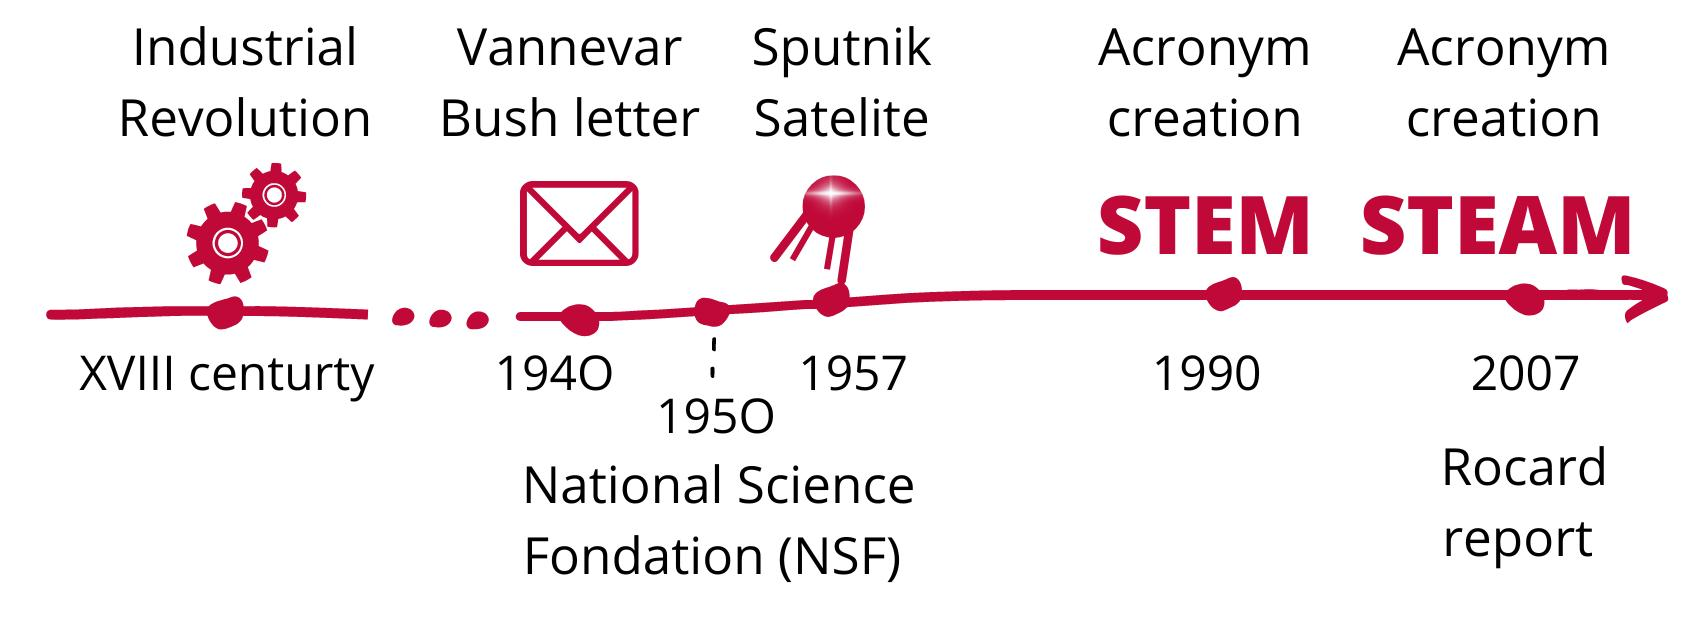
\includegraphics[width=\textwidth]{imagem1.jpg}
 \caption{STEAM education timeline}
 \label{fig1}
 \source{the authors.}
\end{minipage}
\end{figure}

Early as 1940, for example, the engineer Vannevar Bush addressed official letters to the USA president Eisenhower emphasising the urgency of creating educational structures to prepare future scientists foreseeing the prosperity of that country \cite{chesky_introduction_2015}. 

During the cold war (1947–1991), the United States of America (USA) and the Union of Soviet Socialist Republics (USSR) experienced ferocious competition for technological supremacy \cite{chesky_introduction_2015}. Those countries embraced policies aiming at technical, economic, and military development that touched various spheres of society, including education. Educational policies focused efforts – and principally investments – on developing specific scientific and technological careers considered national interest \cite{catterall_brief_2017}.

An essential point was the National Science Foundation (NSF) creation in 1950 – a governmental agency aimed to promote education and research in science and engineering \cite{NSF1950}. Seven years later, the Russian Sputnik-1 satellite was launched into orbit around the Earth. This revolutionary event triggered many USA reactions \cite{perignat_steam_2019}. Among some of these responses, NSF formalised the acronym STEM in 1990 to refer – and principally justify – what became known as an investment “pipeline” in science, technology, engineering, and mathematics \cite{reynolds2009increasing, stephenson_increasing_2022}.

Indeed, the STEM movement was initially justified by economic and military competitiveness \cite{chesky_introduction_2015}. Nevertheless, this movement later progressed to STEM education – an educational approach centred on interdisciplinarity between the areas constituting the acronym \cite{kelley_conceptual_2016}. In this transition, STEM incorporated educational trends and discourses such as active, collaborative, authentic, meaningful, and playful learning \cite{michael_wheres_2006, zosh_accessing_2018}. 

STEM implied educational investment policies narrowed to technical areas \cite{reynolds2009increasing, stephenson_increasing_2022}. In opposition, representatives revindicate against the devaluation in American schools of the areas left out of the acronym. Accordingly, the new acronym STEAM was formalised at the Americans for the Arts-National Policy Roundtable, including A for the arts \cite{perignat_steam_2019}.

Following this, researchers argued that STEAM could be more comprehensive than STEM by encompassing arts and humanities \cite{guyotte_toward_2020}. The same, UNESCO established STEAM as an appropriate approach to achieving Sustainable Development Goals (SDGs) \cite{united2018} while conceiving sustainability as a broader concept that includes social, environmental, and economic aspects \cite{brundtland1987}.

STEM and STEAM have been adopted in many countries and continents. The European Commission, for example, published a report proposing a new pedagogy for the future of Europe with an emphasis on science education \cite{rocarb2007}. Parallelly, those approaches have grown as educational research lines \cite{marin-marin_steam_2021}. \Cref{fig2} shows the number of articles indexed on the Web of Science (WoS) in the category of educational research with the terms STEM or STEAM in its topics (title, abstract, or keywords). We note that research in STEAM is still much less expressive than in STEM. Considering the number of publications in the graph, STEAM represents only 6\%.

\begin{figure}[htbp]
\centering
\begin{minipage}{.8\textwidth}
 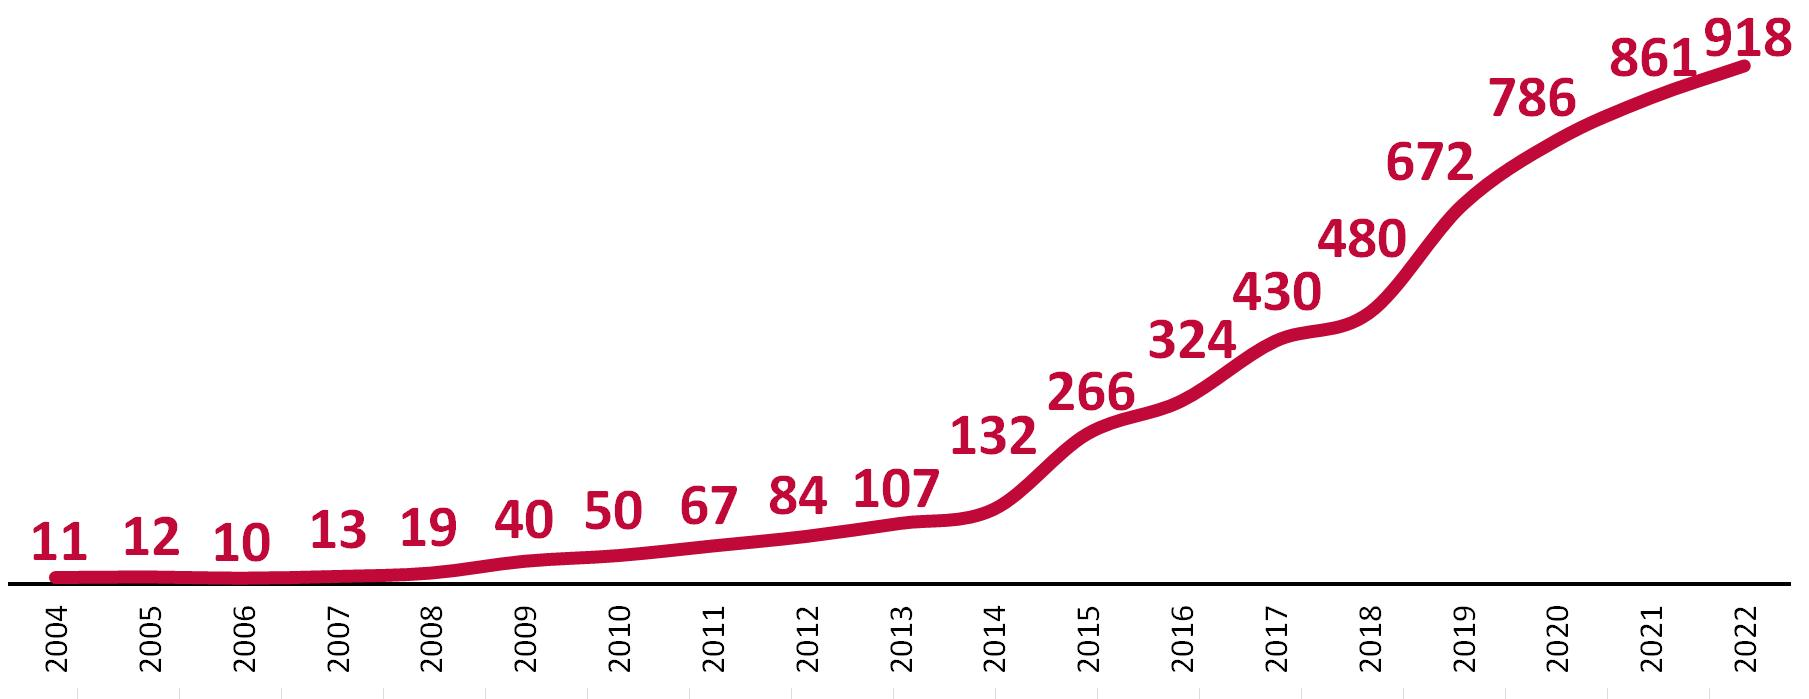
\includegraphics[width=\textwidth]{imagem2.jpg}
 \caption{Amount of articles indexed on Web of Science in the category educational research with the terms STEM or STEAM.}
 \label{fig2}
 \source{the authors.}
\end{minipage}
\end{figure}

The authors of this review clarify their inclinations toward STEAM education vis-à-vis its inclusiveness of arts and humanities. STEAM is more comprehensive in addressing complex issues such as sustainability \cite{rodrigues-silva_stem/steam_2023b, brundtland1987}. Rather than merely fulfilling utilitarian goals and agendas extrinsic from education, we believe STEAM has significant potential to meet subjects’ purposes and those intrinsic to education \cite{biesta_por_2022, rodrigues-silva_stem/steam_2023b}.

\section{What STEAM is not}

We do not intend to define STEAM by its negative, but we are confident that reflecting on what STEAM education is not may contribute to elucidating it. In this direction, we explore the underpinning rationale which supports that STEAM is not an evolution of STEM, a teaching methodology, a synonym of interdisciplinarity, or an attempt to erase the disciplines (based on transdisciplinarity).

\textbf{STEAM is not an evolution of STEM}: STEM and STEAM education are inexorably interconnected because one emerged as a response to the other \cite{perignat_steam_2019}. Additionally, both approaches share interdisciplinary teaching at their core and imply the insertion of engineering and technology pre-college curricula \cite{moore_framework_2014}.

However, if STEAM contains all four areas of the previous acronym, why do some people advocate for STEM over STEAM? There should be differences that justify this positioning. \textcite{khine_creating_2019} explains that some STEM practitioners reject the extension of the acronym, fearing to divert attention (privilege) from technical areas. In this vein, \textcite{clements_stem_2021} warn that broadening the acronym to other knowledge areas will likely weaken the cohesion of STEM education. However, they oversee that perhaps that is precisely what STEAM defensors intended in the first place.

The conflict that motivates STEAM as a response to STEM remains central to their relationship. On the one hand, STEM represents a convergent standpoint of selecting specific areas of knowledge – meaning not including humanistic disciplines. On the other hand, STEAM proposes reinserting arts and humanities into the educational programme. This conflictual relationship allows stating that STEAM is not simply an evolution of STEM because they reflect contradictory philosophies regarding narrowing or broadening the curriculum.

\textbf{STEAM is not a teaching methodology}: STEAM usually endorses active, collaborative, authentic, meaningful, and playful learning \cite{michael_wheres_2006, zosh_accessing_2018}. In parallel, several teaching methodologies are argued to support STEAM in those learning settings. Accordingly, STEAM activities have been developed by teaching methodologies such as Project-Based Learning (PjBL) \cite{lu_project-based_2022}, Problem-Based Learning (PBL), and Inquiry-Based Learning (IBL) \cite{quigley_developing_2017}. Furthermore, reports highlight positive outcomes of STEAM intertwined with playful approaches such as Free play, Game-Based Learning, and Gamification \cite{aurava_expectations_2022, rodrigues2022aamatematicas}.

This plurality of strategies is restricted if STEAM is portrayed as aligned with one specific teaching methodology. Such simplification hinders the dialogue between STEAM practitioners and researchers who envisioned STEAM through different pedagogical strategies. In other moments, STEAM is misguided as a teaching methodology itself. While occupying a place of methodology, STEAM overshadows teaching methodologies that could benefit STEAM with theoretical and empirical knowledge historically constructed on them. Additionally, this misunderstanding generates discredit associated with the feeling that STEAM is just another name for concepts already consolidated in educational research.

In sum, STEAM education should not be restricted to or understood as a teaching methodology. Even though a STEAM activity might be inevitably circumscribed in a specific teaching methodology, various teaching methodologies contribute to various undertakings aiming at the interdisciplinary teaching of STEAM disciplines (we will differentiate STEAM education from STEAM activity later).

\textbf{STEAM is not a synonym for interdisciplinarity}: First, we clarify that disciplines represent branches of knowledge that can be distinguished from other knowledge areas according to different epistemology, theories, and methods. Disciplines or knowledge areas are comprehensible parts of knowledge that permit its organisation \cite{florentino_disciplinaridade_2015}. Following, we query the various forms they can relate to each other. As shown in \Cref{fig3}, the word discipline is commonly accompanied by the prefixes intra, cross, multi, inter, and trans. Those modifiers express concepts widely used, and frequently misunderstood, in the literature.

\begin{figure}[htbp]
\centering
\begin{minipage}{.9\textwidth}
 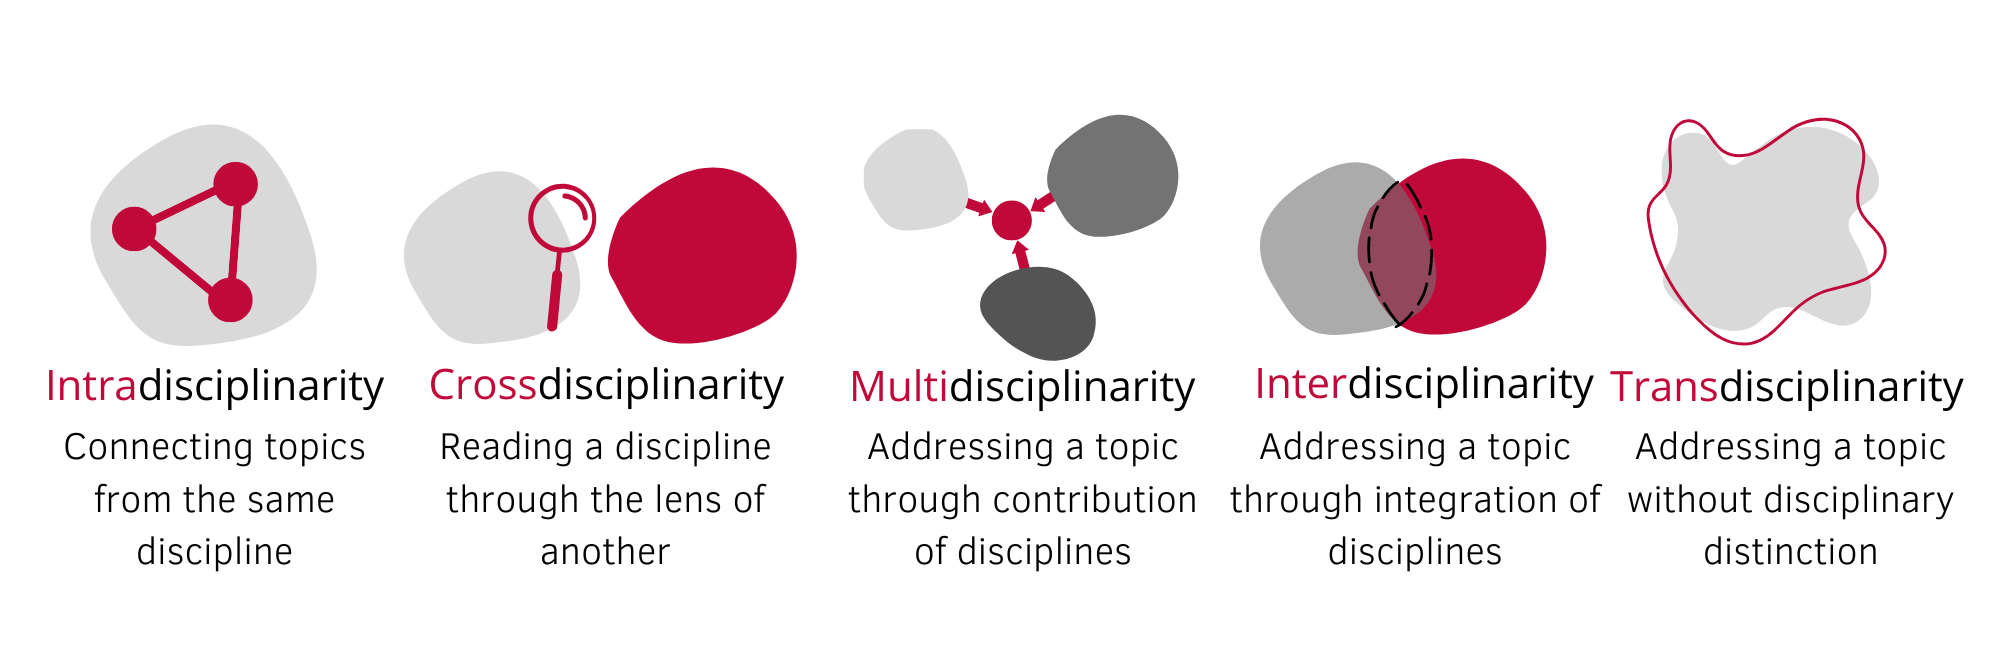
\includegraphics[width=\textwidth]{Fig3.png}
 \caption{Disciplinary relations}
 \label{fig3}
 \source{the authors.}
\end{minipage}
\end{figure}

Intradisciplinarity addresses the connection of topics within the scope of the same discipline. Cross-disciplinarity observes a topic from one discipline, taking the perspective of another. Multidisciplinarity means that disciplines separately contribute to understanding a topic or problem. Interdisciplinarity concerns integrating disciplines so that there is dialogue through them and their interspaces or intersections \cite{danermark_applied_2019}. Differently, transdisciplinarity aims to synthesise knowledge so that a topic can be holistically comprehended.

Repeatedly, multi, inter, and transdisciplinarity are interchangeably enunciated so that their meaning differences are emptied. \textcite{politi2019interdisciplinarity} argues that those three concepts represent progressive stages of disciplinarity integration – with transdisciplinarity referring to the latest stage of this process. Nonetheless, this assumption of one integration process carries incompatibilities.

In interdisciplinarity, discipline borders are momentaneously crossed to highlight their intersections. This way, disciplines can be integrated through dialogue that provides understanding within and synergistically beyond the disciplines’ original scope. Consequently, interdisciplinarity place disciplines as essential substrates for integration, and they are strengthened by contact with each other \cite{boufleuer_interdisciplinaridade_2020, florentino_disciplinaridade_2015}.

Conversely, transdisciplinarity seeks to transcend the boundaries of disciplines while considering a holistic whole that would better address complex issues \cite{guyotte_steam_2014}. In transdisciplinarity, the focus remains on the problem without discerning individual disciplines and outlining intersections. Hence, instead of a superior stage of interdisciplinarity, transdisciplinarity represents a different, perhaps opposing concept.

Importantly, interdisciplinarity and STEAM are not synonymous because the former refers to the dialogue between disciplines (in general), and the latter consists of such dialogue considering the group of disciplines described in the acronym. Consequently, beyond interdisciplinarity, STEAM implies a curriculum modernisation considering relevant knowledge areas introducing disciplines traditionally overseen at pre-college levels – technology and engineering \cite{moore_framework_2014}.

\textbf{STEAM is not an attempt to erase the disciplines}: Initially, listing disciplines in the acronym of an educational approach that aims at integration possibly seem confusing. At the same time, it can sound reasonable wondering the creation of one holistic macro discipline instead of mentioning discrete knowledge areas.

Indeed, students are likely to learn holistically from experiences in activities wherein they are unaware of which knowledge areas are being applied – as suggested in transdisciplinarity \cite{strobel_role_2013}. Notwithstanding, interdisciplinary education is distinctive from everyday learning precisely when offering insights from the disciplines. In this sense, interdisciplinarity fosters students’ reflection on experiences to build consciousness about the disciplines, strengthen disciplinary knowledge, and explore their intersection \cite{florentino_disciplinaridade_2015, pearson_national_2017}. In other words, while transdisciplinarity might result in some learning from experience, interdisciplinarity further explores those experiences by explicitly addressing the disciplines involved.

Consequently, we argue that interdisciplinarity is a central aspect of STEAM. In order to be educational, STEAM requires an understanding of each discipline and its intersections \cite{thibaut_integrated_2018}. In STEAM, teachers have to teach \cite{biesta_por_2022} – they encourage reflection on experiences and convey knowledge students would not recognise as such from merely experiencing an activity. Hence, STEAM is not an attempt to erase the disciplines. Contrarily, this educational approach is firmly grounded in the disciplines that constitute it.



\section{STEAM education definition}

First, we evoke the five general rules of definition: exclusion of the negative, adequacy, clarity, non-circularity, and brevity \cite{machlarz2011general} Among them, we recall the rule of exclusion of the negative states that definitions must not come from the negative. Therefore, we elucidate that the considerations on the negative of STEAM presented so far helped to understand but do not define it.

Next, we articulate two conditions for STEAM education – interdisciplinarity and the knowledge areas of science, technology, engineering, arts/humanities, and mathematics. First, we outline that recalling \textbf{STEAM disciplines means distinctively listing the acronym’s knowledge areas}. Next, we highlight that, on the one hand, although interdisciplinarity is central to STEAM, it does not encompass the whole idea of STEAM regarding setting a group of disciplines as pertinent to current and future society. On the other hand, only establishing a group of STEAM disciplines does not configure STEAM education – an educational approach that aims to integrate those disciplines.

Therefore, these conditions are necessary and sufficient (if together) to define STEAM. Accordingly, \textbf{STEAM education is an educational approach that promotes interdisciplinary teaching of the STEAM disciplines in its set of practices}.

Further exploring this definition, it appreciates all the letters of the acronym in their quality of knowledge area. Researchers defend that teaching in STEAM should not hierarchise the disciplines. In other words, one area should not be reduced to an educational tool in service to teach other \cite{mejias_trouble_2021}.

Moreover, we remark that STEAM education means teaching all areas of the acronym. In this respect, \textcite{toma_stem_2021} criticise that the literature in STEM/STEAM is too pretentious for promoting a set of areas in the acronyms if practitioners are content with the requirement to integrate at least two areas. However, these authors disregarded that education is not attained with a single session or activity. In this sense, it is worth differentiating STEAM activity from STEAM education. STEAM activity or lesson is an educational practice aligned with, but that does not necessarily fulfill all conditions of STEAM because it is a single episode of STEAM education. Thus, a \textbf{STEAM activity or lesson is a practice of interdisciplinary teaching of at least two STEAM disciplines}.

STEAM activities should contemplate at least two areas to ensure interdisciplinarity. In this sense, a STEAM activity has to be planned according to the pertinence of STEAM disciplines regarding a particular topic or problem. For the same reason, it may be appropriate for one discipline to be central and the other to play complementary roles in a specific activity. At this level, interdisciplinary didactic planning should prioritise students’ learning benefits rather than desperately forcing the presence of all STEAM disciplines \cite{pearson_national_2017, thibaut_integrated_2018} or misleadingly pursuing equilibrated development between the areas.

Especially in empirical studies, researchers explore STEAM activities – which naturally have particular settings – and tend to extrapolate the specific characterisation of those activities to STEAM education. When brevity is abandoned in the STEAM definition, it generates disagreement due to unnecessary restrictions. For example, authenticity – addressing real-world problems – might be vital in several STEAM activities \cite{strobel_role_2013}. Nevertheless, a definition of STEAM Education that includes authenticity would conflict with, for example, playful learning, whose activities are embedded in imagination, fantasy, and mythical contexts \cite{rodrigues-silva_educacion_2023a}.

In this sense, besides brevity, the definition of STEAM education presented here complies with the rule of adequacy because it suits the defined object and nothing else. Furthermore, it is clear and non-circular because the term to be defined is not in the body of the definition. Finally, we argue that instead of changing and stretching the definition of STEAM to accommodate particular activities, we propose envisioning the breadth of STEAM education coherent from various teaching methodologies and educational purposes.

\section{STEAM education framework}

Characterising differs from defining regarding its no pretension of reaching exhaustion \cite{machlarz2011general}. Thus, STEAM is usually characterised by active, collaborative, authentic, meaningful, and playful teaching and learning \cite{lin_effect_2021, ortiz-revilla_mirada_2021, quigley_developing_2017}. Undoubtedly, those configurations and teaching and learning are relevant to STEAM education since literature has pointed out them as effective strategies for education on many occasions \cite{michael_wheres_2006}.

Briefly mentioning, researchers propose STEAM activities aiming at the development of creativity \cite{aguilera_stem_2021}, critical thinking \cite{bassachs_fostering_2020}, engineering thinking \cite{rodrigues2023}, and food literacy \cite{silva-hormazabal_conectando_2022}. In this line, STEAM might be appropriate to address various objectives intrinsic to education, from the subject \cite{biesta_risking_2020}, and aligned with international agendas of social interest, such as Education for Sustainability \cite{guyotte_toward_2020, vasquez_education_2021}.

Considering all that, we propose in \Cref{fig4} a conceptual framework of STEAM in a table format incorporating STEAM definition (exhaustive) and characterisation (non-exhaustive). From this picturisation, we remark that the tabletop – the part that makes the table a table – represents STEAM’s two sufficient and necessary conditions. Differently, teaching methodologies and objectives are closely related to specific STEAM activities instead of defining STEAM as an educational approach. Therefore, we represent teaching and learning configurations as the table legs – although significant, missing one table leg does not disqualify it as a table. Eventually, we represent educational objectives as constructions on the table – they are supported by the whole table.

\begin{figure}[htbp]
\centering
\begin{minipage}{.8\textwidth}
 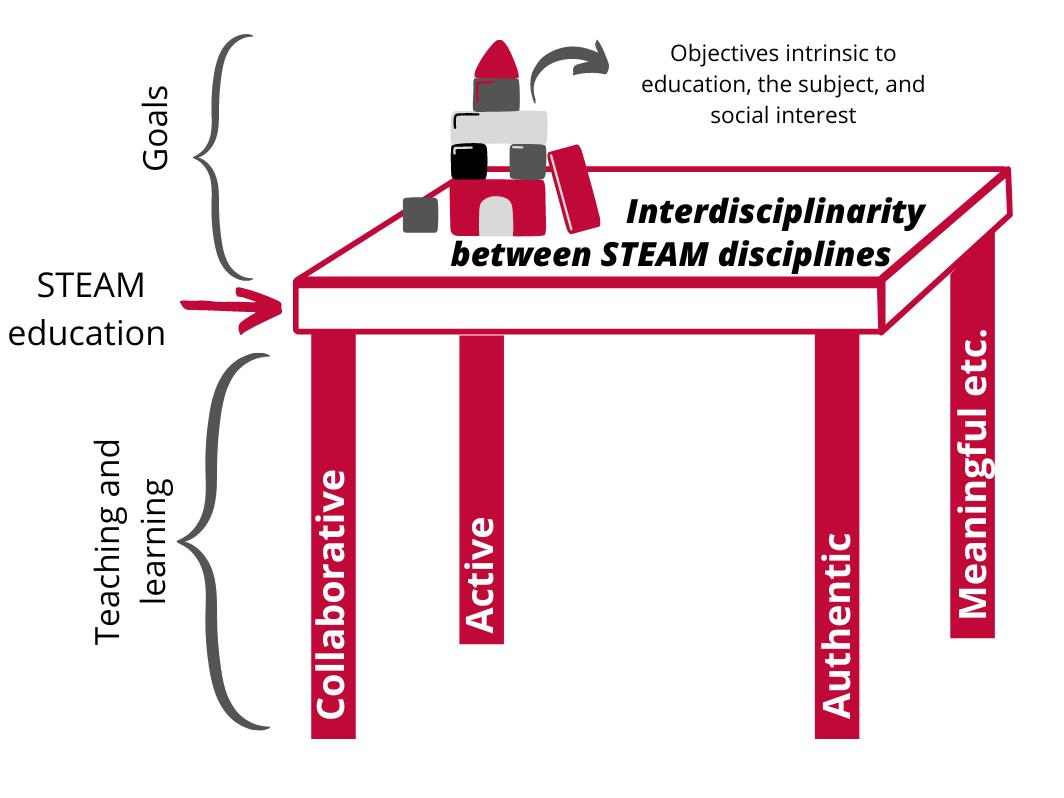
\includegraphics[width=\textwidth]{imagem4.jpg}
 \caption{Conceptual framework of STEAM education}
 \label{fig4}
 \source{the authors.}
\end{minipage}
\end{figure}

Notably, teaching and learning configurations and objectives are accompanied by an “etcetera” to reaffirm the non-intention of exhaustion in the characterisation of STEAM education.



\section{Conclusions}

As \cite{marin-marin_steam_2021} evidenced, STEAM is a recent research line still under construction. Accordingly, this review pointed out some STEAM definition incongruences which may be problematic to its understanding and practice \cite{perignat_steam_2019}. Therefore, we inquired about what is (and what is not) STEAM education.

In response, this study elucidated that STEAM is not a simple evolution of STEM nor a teaching methodology. We expressed rationalities underpinning STEAM as an interdisciplinary approach – strongly supported by the disciplines and their intersections – instead of pursuing transdisciplinarity, where knowledge remains undefined in a holistic whole.

We could differentiate STEAM disciplines (list of the five knowledge areas), STEAM activities (interdisciplinary teaching unity of at least two STEAM disciplines), and STEAM education (educational approach of interdisciplinarity between all STEAM disciplines).

Finally, we proposed a STEAM conceptual framework in a table format. This framework contributes by emphasising the essential aspects of STEAM definition (tabletop). This characterisation mentions some teaching methodologies and educational objectives but is not restrictive, asserting the multiplicity of doings of education, paradigms, and methodologies already existing in the literature.

The conclusions from this review impact STEAM practice calling attention to teaching as an addition that makes this approach distinctively education in regard to everyday learning (knowledge diffused). While stressing interdisciplinarity, we assert the importance of further exploring students’ experiences by explicitly addressing the disciplines and their intersections. Concerning teacher education, on the one hand, STEAM requires teacher professional development that enhances agency on a plurality of teaching methodologies associated with STEAM to achieve educational goals. On the other hand, individual STEAM activities require proper lesson planning, including the ability to select appropriate disciplines and intentionally develop them. At the same time, STEAM education remarks the need to articulate all STEAM disciplines, including technology and engineering, that knowledge areas traditionally missing at pre-college levels.












\printbibliography\label{sec-bib}
% if the text is not in Portuguese, it might be necessary to use the code below instead to print the correct ABNT abbreviations [s.n.], [s.l.]
%\begin{portuguese}
%\printbibliography[title={Bibliography}]
%\end{portuguese}


%full list: conceptualization,datacuration,formalanalysis,funding,investigation,methodology,projadm,resources,software,supervision,validation,visualization,writing,review
\begin{contributors}[sec-contributors]
\authorcontribution{Jefferson Rodrigues-Silva}[conceptualization,datacuration,formalanalysis,investigation,methodology,visualization,review]
\authorcontribution{Ángel Alsina}[conceptualization,investigation,methodology,supervision,validation,review]
\end{contributors}





\end{document}

